\icode{E-MM-SI-L2-261014-001}
光子有能量，也有动量，它也遵守有关动量的规律。如图所示，真空中有一“\(\infty\)”字形装置可绕通过横杆中点的竖直轴\(OO^\prime\)在水平面内灵活地转动，其中左边是圆形黑纸片，右边是和左边大小、质量均相同的圆形白纸片。当用平行白光垂直照射这两个圆面时，关于此装置开始时转动情况（俯视）的下列说法中正确的是\paren[]

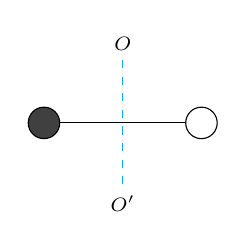
\begin{tikzpicture}[font=\scriptsize]
	\draw (-1,0)--(1,0);
	\draw[dashed,cyan] (0,.8)node[above,black]{\(O\)}--(0,-.8)node[below,black]{\(O^\prime\)};
	\draw[fill=gray!50!black] (-1,0) circle(.2);
	\draw[fill=white] (1,0) circle(.2);
\end{tikzpicture}
\begin{choices}
	\item 顺时针方向转动
	\item 逆时针方向转动
	\item 都有可能
	\item 不会转动
\end{choices}	